\section{Architecture and Implementation Details}
\label{sect:architecture}

Our system runs on a cluster of Linux machines with Xen-based VMs and
an open-source package for the distributed file system  called QFS~\cite{michael2013}. 
%to %manage  the physical disk storage. 
All data needed for the backup service including snapshot and  metadata data
%and snapshot data for backup purposes, 
resides in this distributed file system. 
One physical node hosts tens of VMs, each of which accesses its virtual machine disk image through the
virtual block device driver (called TapDisk\cite{Warfield2005} in Xen).

\subsection{ Components of a cluster node } 
As depicted in Figure~\ref{fig:arch_vm}, 
there are four key service components running on each cluster
node  for supporting backup and deduplication: 
1) a virtual block device driver, 2) a snapshot deduplication component,
3) an append store client to store  and access snapshot data,
and 4)  a PDS client to support PDS metadata access. 

We use the virtual device driver in Xen that employs a bitmap to track the changes 
that have been made to the virtual disk.
Every bit in the bitmap represents a fixed-sized (2MB) region called a \textit{segment}, indicating whether the segment
has been modified since last backup. 
Segments are further divided into variable-sized chunks (average 4KB) 
using a content-based chunking algorithm~\cite{frame05}, 
which brings the opportunity of fine-grained deduplication.
When the VM issues a disk write, the dirty bit for the corresponding segment is set
and this indicates such a segments needs to be checked during snapshot backup. 
After the snapshot backup is finished, the driver resets the dirty bit map to a clean state.
For data modification during backup, copy-on-write protection is set so that backup can continue to
copy  a specific version while new changes are recorded.
%copies a frozen version while the modification can still carry on.

The representation of each snapshot has  a two-level index data structure.
The snapshot meta data (called snapshot recipe) contains a list of segments, each of which contains segment
metadata of its chunks (called segment recipe).
In snapshot and segment recipes, 
the data structures  include references to the actual data location to eliminate the need for additional indirection.

\begin{figure}[htbp]
    \centering
    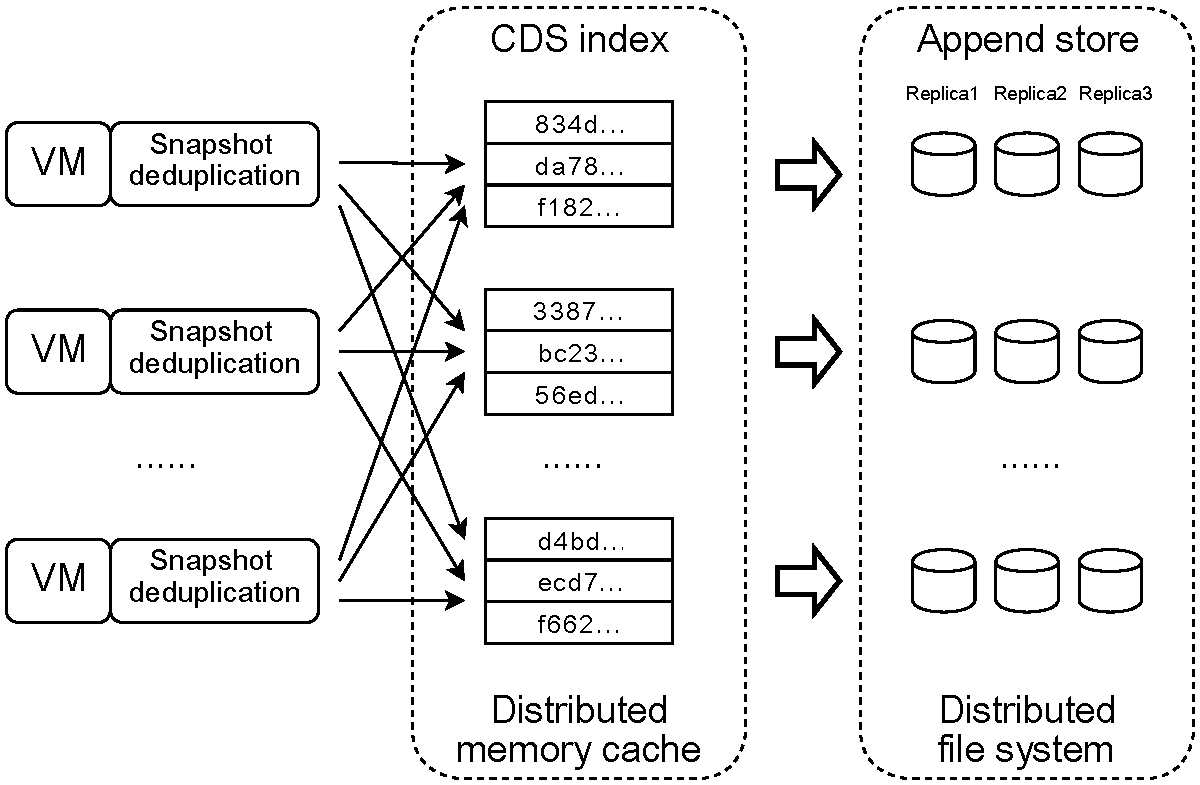
\includegraphics[width=2.75in]{images/socc_arch_cluster}
    \caption{System architecture and data flow during snapshot backup}
    \label{fig:arch_vm}
\end{figure}

\subsection{A VM-centric snapshot store for backup data}
\label{sect:store}
We build the snapshot storage on the top of a distributed file system.
Following the VM-centric idea for the purpose of fault isolation,
each VM has its own snapshot store, containing new data chunks which are considered
to be non-duplicates.
There is also a special store containing all PDS chunks shared among different VMs.
As shown in Figure~\ref{fig:as_arch}, we explain the data structure of the snapshot stores as follows.
\begin{figure}[htbp]
  \centering
  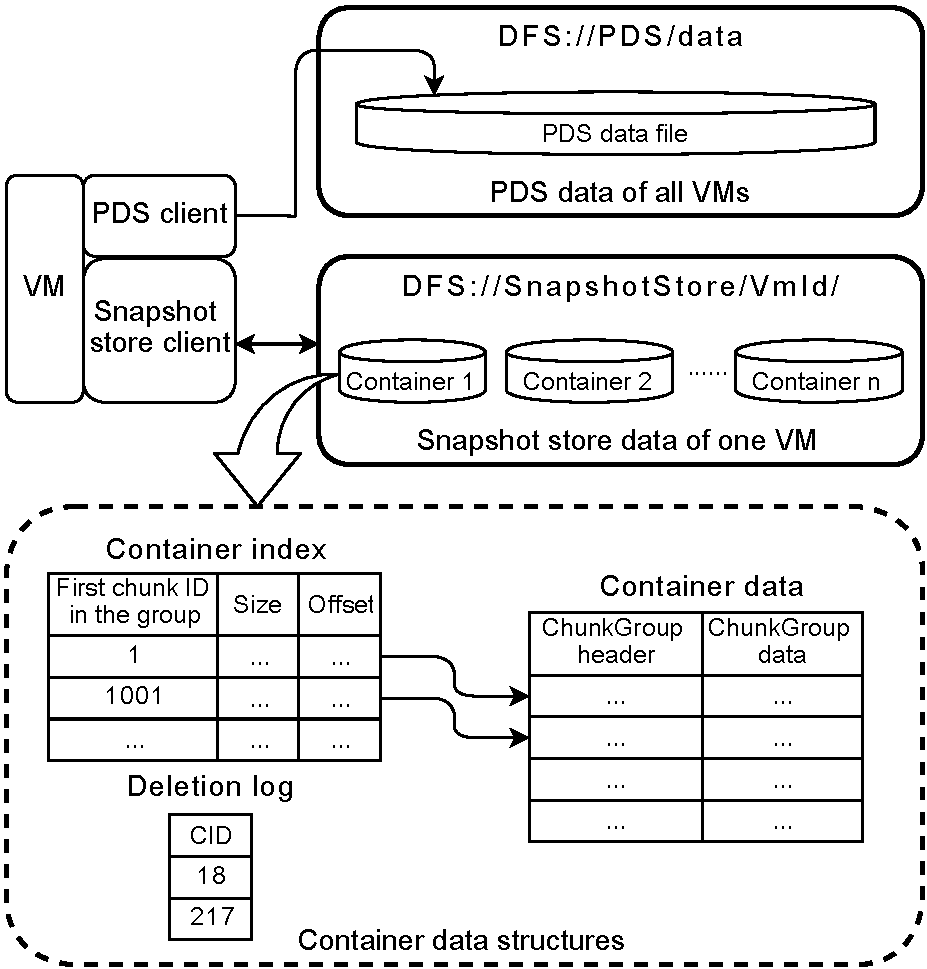
\includegraphics[width=2.75in]{images/sstore_arch}
  \caption{Data structure of a VM snapshot store.}
  \label{fig:as_arch}
\end{figure}

%\begin{itemize}
%\item
PDS chunks are stored in one PDS file. 
Each reference to a PDS data chunk in the PDS index is the offset within the PDS file.
%There is an option to use a data structure similar to the non-PDS store. We opt
%for the simpler format because
Additional compression is not applied because PDS chunks have less spatial locality in data access. 
For the data sets we have tested, we only observed very limited spatial locality 
among popular data chunks. On average the number of consecutive PDS index hits is lower than 7.
Thus it is not so effective to group a large number of chunks as a compression and data fetch unit. 
For the same reason, we decide not to take the sampled index approach~\cite{Guo2011} 
for detecting duplicates from PDS as limited spatial locality is not sufficient to enable
effective prefetching for sampled indexing.

PDS data is re-calculated periodically, but 
the total data size is small.  When
a new PDS data  set is computed, in-memory PDS index is replaced, but 
the PDS file on the disk appends the  new PDS data identified and the growth of this file is very slow. 
The old data is not removed because they can still be referenced by the existing snapshots. 
A periodic cleanup is conducted  to remove unused PDS chunks (e.g. every few months). 

%\end{itemize}

For non PDS data, the snapshot store of a VM is  divided into a set of containers and 
each container is approximately 1GB. 
The reason for dividing the snapshot into containers is to simplify the compaction process
conducted periodically. As discussed later, data chunks are deleted from old snapshots
and chunks without any reference from other snapshots can be removed by this compaction process.
By limiting the size of a container, we can effectively control the length of each round of compaction.
The compaction  routine can work on one container at a time and move the in-use data chunks to another container. 

Each non-PDS data container is further divided into a set of chunk data groups. Each chunk group is composed of
a set of data chunks and is the basic unit in data access and retrieval. 
In writing a chunk during backup, the system accumulates data chunks and stores the entire
group as a unit after compression. This  compression can reduce data by several times  in our tested applications.
When accessing a particular chunk, its chunk group is retrieved from the storage
and decompressed. Given the high spatial locality and usefulness of prefetching  in 
snapshot chunk accessing~\cite{Guo2011,foundation08},
retrieval of  a data chunk  group naturally works well with prefetching. 
A  typical chunk group contains 1000 chunks in our experiment.
% with an average size of 200-600 chunks.

%\item
Each data container is represented by three files in the DFS:
1) the container data file holds the actual content, 
2) the container index file is responsible for translating a data reference
into its location within a container, and 
3) a chunk deletion log file records all the deletion requests within  the container.

%\item
A non-PDS data chunk reference stored in the index of snapshot recipes
is composed of two parts: a container ID with 2 bytes and a local chunk ID with 6 bytes.
Each container maintains a local  chunk counter and assigns the current number 
as a chunk ID  when  a new chunk is added to this  container. 
Since data chunks are always appended to a snapshot store during backup, 
local chunk IDs are monotonically increasing.
When a snapshot chunk is to be accessed, the snapshot recipe contains a reference pointing to  a data chunk
in the PDS store or in a non-PDS VM snapshot  store. 
Using  a container ID, the corresponding container index file of this VM is accessed and 
the chunk group is identified using a simple chunk ID range search. Once the chunk group is loaded to memory, 
its header contains the exact offset of the corresponding chunk ID and the content is then accessed from the memory buffer.

%\item


The snapshot  store supports three API calls:
%\begin{itemize}

%\item
\noindent\textbf{Append()}. 
For PDS data, the chunk is appended to the end of the PDS file and the offset is returned as the  reference.
For non-PDS data, this call places a chunk into 
the snapshot store and returns a reference to be stored in 
the recipe metadata of a snapshot. 
The write requests to append data chunks to a VM store are accumulated at the client side. 
When the number of write requests reaches a fixed group size, the snapshot store client compresses
the accumulated   chunk group, adds a chunk group index  to the beginning of the group, and then
appends the header and data  to the corresponding VM file.
A new container  index entry is also created for each chunk group and is written to the corresponding
container index file.

%\item
\noindent\textbf{Get()}.
The fetch operation for the PDS data chunk is straightforward since each reference contains 
the file offset, and the size of a PDS chunk is available from a segment recipe.
We also maintain a small data cache for the PDS data service to speedup common data fetching.

To read a non-PDS chunk using its reference with container ID and local chunk ID,  the snapshot store client first loads the
corresponding VM's container index file specified by the container ID, then searches the chunk
groups  using their  chunk ID coverage.
After that, it reads the identified chunk group from DFS, decompresses it, and seeks to the exact chunk data 
specified by the chunk ID. 
Finally, the client updates its internal chunk data cache with the newly loaded content to 
anticipate future sequential reads.

%\item
\noindent\textbf{Delete()}.
Chunk deletion occurs when a snapshot expires or gets deleted explicitly by a user and we discuss this in more details in next
subsection.
%(we will discuss the snapshot deletion in detail in the following subsection).
When deletion requests are issued for a specific container,
those requests are simply recorded into the  container's deletion log initially and thus  a lazy
deletion strategy is exercised.
Once local chunk IDs appear in
the deletion log, they will not be referenced by any future snapshot and can be safely deleted when needed. 
This is ensured because we only dedup against the direct parent of a snapshot, so the deleted snapshot's blocks
will only be used if they also exist in other snapshots.
Periodically, the snapshot  store picks those containers with an excessive
number of deletion requests to  compact and  reclaim the corresponding disk space. 
During compaction, the snapshot store creates a new container (with the same container ID) to replace the 
existing one. This is done by sequentially scanning the old container, copying all the chunks that are not 
found in the deletion log to the new container, and creating new chunk groups and indices. 
Every local chunk ID however is directly copied rather than re-generated. This
process leaves holes in the CID values, but preserves the order and IDs of chunks.
As a result, all data references stored 
in recipes are permanent and stable, and the data reading process
is as efficient as before. Maintaining the stability of chunk IDs also ensures that recipes do not
depend directly on physical storage locations, which simplifies data migration.
%\end{itemize}


\subsection{ VM-centric Approximate Snapshot Deletion with Leak Repair}
\label{sect:delete}


\begin{figure}[htbp]
  \centering
  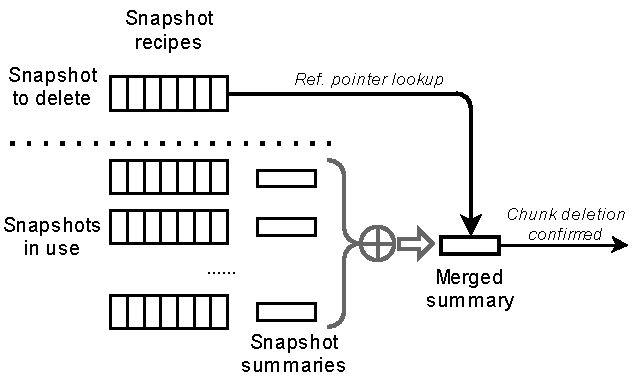
\epsfig{file=images/deletion.pdf, width=3in}
  \caption{Approximate deletion}
  \label{fig:deletion_flow}
\end{figure}

In a busy VM cluster, snapshot deletions can occur frequently.
Deduplication complicates the deletion process because space saving relies on the sharing of data
and it requires the global references to deleted chunks to be identified before  they can be safely removed.
While we can use the mark-and-sweep technique~\cite{Guo2011}, 
it takes significant resources to conduct this process every time there is a snapshot deletion.
In the case of Alibaba, snapshot backup is conducted automatically and there are 
about 10 snapshot stored for every VM customer. When there is
a new snapshot created every day,  there will be a snapshot expired every day to maintain
balanced storage use. 

We seek a fast solution with low resource usage to delete snapshots and
our VM-centric design simplifies the deletion process. 
Since PDS is small and separated, we can focus on  unreferenced non-PDS chunks within each VM. 
%The PDS data chunks are commonly shared among all VMs and we do not consider them
%during snapshot deletion.  The selection of PDS data chunks is updated periodically independent of snapshot deletion process.
Another resource-saving strategy we propose is
an {\em approximate} deletion strategy to trade deletion accuracy for
speed and resource usage. Our method sacrifices a small percent of storage leakage
to efficiently identify unused chunks.
The algorithm contains three aspects.

\begin{itemize}
\item {\bf Computation for snapshot reference summary.}
Every time there is a new snapshot created,
we compute a Bloom-filter with $z$ bits as the reference summary vector for all non-PDS chunks used 
in this snapshot,
the items we put into summary vector are all the references that are used in its snapshot and segment recipes.
Foe each VM we preset the vector size according to  estimation of VM image size,
given $h$ snapshots stored for a VM, there are $h$ summary vectors maintained.

\item {\bf Approximate deletion with fast summary comparison.}
When there is a snapshot deletion,  
we need to identify if  chunks to be deleted from that snapshot
are still referenced by other snapshots. 
This is done approximately and quickly by comparing the 
reference of deleted chunks  with
the merged Bloom-filter reference summary of other live snapshots.
The merging of live snapshot Bloom-filter bits uses the bitwise OR operator 
and the merged vector still takes $z$ bits.
Since the number of live snapshots $h$ is limited for
each VM, 
the time and memory cost of this comparison is small, linear to the number of chunks to be deleted.

If a chunk's reference is not found in the merged summary vector, we are sure that
this chunk is not used by any live snapshots, thus can be deleted safely.
However, among all the chunks to be deleted, 
there are a small percentage of unused chunks  which
are misjudged as  being in use, resulting in storage leakage.

\item {\bf Periodic repair of leakage}.
%[exlpain why second Bloom filter, why scan append store]
Leakage repair is conducted periodically to fix the above approximation error.
This procedure compares the live chunks for each VM with what are truly used in the VM snapshot recipes.
That requires a scan of all the metadata in a single VM backup. Since it is a VM-specific procedure 
the space and time cost is relatively small compared to the traditional mark-and-sweep procedure~\cite{Guo2011} which scans snapshot 
chunks from all VMs.
For example,
consider each reference consumes 8 bytes plus  1 mark bit, a VM that has 40GB backup data with about
10 million chunks will need less than 85MB of memory to complete a VM-specific mark-and-sweep process.
\end{itemize}

%{\bf Discussion}
We now estimate the size of storage leakage and how often leak repair needs to be conducted.
Assume that  a VM keeps $h$ snapshots in the backup storage, creates and deletes one snapshot
every day. Let $u$ be the total number of chunks brought by the initial backup for a VM, $\Delta u$ be the average
number of additional chunks added from one snapshot to the next snapshot version. Then the total number of 
chunks stored in a VM's snapshot store is about:
\[
U = u + (h-1)\Delta u.
\]

Each Bloom filter vector has  $z$ bits for each snapshot and let $j$ be the number of hash functions used by the
Bloom filter.  Notice that a chunk may appear multiple times in these summary vectors; however, this should not 
increase the probability of being a 0 bit in all $h$ summary vectors.
Thus the probability that a particular bit is 0  in all $h$ summary vectors is  
$(1- \frac{1}{z}) ^{j U}$. 
Then the misjudgment rate of being in use  is: 
\begin{equation}
\label{eq:falserate}
\epsilon = (1-(1-\frac{1}{z})^{jU})^j.
\end{equation}

For each snapshot deletion, the number of chunks to be deleted is nearly identical to the number of
newly added chunks $\Delta u$. 
Let $R$ be the total number of runs of approximate deletion between two consecutive 
repairs. We estimate  the total leakage $L$ after $R$ runs as:
\[
L = R \epsilon \Delta u.
\]

When leakage ratio $L/U$ exceeds a pre-defined threshold $\tau$, we derive the condition to execute a leak repair as:

\begin{equation}
\label{eq:leakrepair}
\frac{L}{U} = \frac{R \Delta u \epsilon}{u+(h-1)\Delta u } > \tau 
\Longrightarrow R > \frac{\tau}{\epsilon}\times\frac{u + (h-1)\Delta u}{\Delta u}.
\end{equation}

For example in our tested dataset,  
each VM keeps $h=10$ snapshots and each snapshot adds
about 0.1-5\% of new data. Thus we take ${\Delta u}/{u} \approx 0.025$. For a 40GB snapshot, $u\approx  10$ million.
Then $U=12.25$ million.
We choose  $\epsilon = 0.01$ and $\tau=0.05$.  From Equation~\ref{eq:falserate}, 
each summary vector requires $z=10U=122.5$ million bits or 15MB. From Equation~\ref{eq:leakrepair}, 
leak repair should be triggered once for every R=245 runs of approximate deletion. 
When one machine hosts 25 VMs and there is one snapshot deletion per day per VM, there would be 
only one full leak repair for one physical machine scheduled for every 9.8 days. 
If $\tau = 0.1$ then leakage repair would occur every 19.6 days.
Each repair uses less than 90MB memory on average
and takes a short period of time.

